\BTTN
\begin{ex}
 \immini{Cho hàm số $f(x)$ có bảng biến thiên như hình bên. Hàm số đã cho đồng biến trên khoảng nào dưới đây?
 \choice
 {\True $(0;1)$}
 {$(2;+\infty)$}
 {$(1;+\infty)$}
 {$(-1;1)$}}{
 \begin{tikzpicture}
 \tkzTabInit[nocadre=false,lgt=1.2,espcl=1.5,deltacl=0.6]
 {$x$ /0.6,$y'$ /0.6,$y$ /2}
 {$-\infty$,$-1$,$0$,$1$,$+\infty$}
 \tkzTabLine{,+,$0$,-,$0$,+,$0$,-,}
 \tkzTabVar{-/$-\infty$, +/$4$,-/$1$,+/$4$,-/$-\infty$}
 \begin{scope}[on background layer]\path[white]node{MDD-122};\end{scope}
 \end{tikzpicture}}	\loigiai{
 Dựa vào bảng biến thiên ta thấy hàm số đồng biến trong $(0;1)$.
 }
\end{ex}
\begin{ex}
 Cho hàm số $y=f(x)$ xác định trên $\mathbb{R}\backslash\{2\}$, liên tục trên mỗi khoảng xác định và có bảng biến thiên như sau:
 \begin{center}
 \begin{tikzpicture}
 \tikzset{double style/.append style = {draw=\tkzTabDefaultWritingColor,double=\tkzTabDefaultBackgroundColor,double distance=2pt}}
 \tkzTab
 [lgt=1.2,espcl=3] % tùy chọn
 {$x$/.7, $f’(x)$/0.7, $f(x)$/2} % cột đầu tiên
 {$-\infty$, $2$, $+\infty$} % hàng 1 cột 2
 {,-,d,-,} % hàng 2 cột 2
 {+/ $1$, -D+/ $-\infty$ / $+\infty$, -/ $1$} % hàng 3 cột 2
 \end{tikzpicture}
 \end{center}
 Trong các khẳng định sau, khẳng định nào đúng?
 \choice
 {Hàm số nghịch biến với mọi $x\neq2$}
 {Hàm số nghịch biến trên tập $\mathbb{R}\backslash\{2\}$}
 {\True Hàm số nghịch biến trên mỗi khảng $(-\infty;2)\mbox{ và }(2;+\infty)$}
 {Hàm số đồng biến trên mỗi khảng $(-\infty;2)\mbox{ và }(2;+\infty)$}
 \loigiai{
 Từ bảng biến thiên, ta thấy $y'<0\ \ \forall x\neq2$.\\
 Suy ra, hàm số nghịch biến trên mỗi khoảng xác định.
 }
\end{ex}
\begin{ex}%[Câu 7]%[2D1N2-2]
 \immini{Cho hàm số $y=f(x)$ xác định trên $\mathbb{R}$ và có bảng biến thiên như hình vẽ bên. Hàm số $y=f(x)$ đạt cực đại tại
 \choice
 { \True $x=10$}
 { $x=8$}
 { $x=12$}
 { $x=17$}}{
 \begin{tikzpicture}
 \tkzTabInit[nocadre=false, lgt=1, espcl=2]
 {$x$ /0.6,$y'$ /0.7,$y$ /1.7}
 {$-\infty$,$10$,$12$,$+\infty$}
 \tkzTabLine{,+,0,-,0,+,}
 \tkzTabVar{-/$-\infty$ ,+/$-3$, -/ $3$ /, +/$-\infty$ /}
 \end{tikzpicture}}
 \loigiai{
 Dựa vào bảng biến thiên ta thấy hàm số đạt cực đại tại $x=10$.
 }
\end{ex}
\begin{ex}
 Hàm số $y=x^3-3x^2+2$ nghịch biến trên khoảng nào trong các khoảng sau đây?
 \choice
 {$(2;+\infty)$}
 {$(-\infty;0)$}
 {$(-\infty;+\infty)$}
 {\True $(0;2)$}
 \loigiai{
 Hàm số có tập xác định $\mathscr{D}=\mathbb{R}$.\\
 $y'=3x^2-6x$, $y'=0\Leftrightarrow \hoac{x &= 0 \\ x &= 2.}$\\
 Với $x=0$, $y=2$; với $x=2$, $y=-2$. Ta có bảng biến thiên sau
 \begin{center}
 \begin{tikzpicture}[scale=1, font=\footnotesize, line join=round, line cap=round, >=stealth]
 \tkzTabInit[nocadre=false,lgt=1.2,espcl=2.5,deltacl=0.6]{$x$/0.6,$y’$/0.6,$y$/2}{$-\infty$,0,2,$+\infty$}
 \tkzTabLine{,+,0,-,0,+,}
 \tkzTabVar{-/$-\infty$,+/$2$,-/$-2$,+/$+\infty$}
 \end{tikzpicture}
 \end{center}
 Từ đó ta được hàm số nghịch biến trên $(0;2)$.
 }
\end{ex}
\begin{ex}
 Trong các hàm số sau, hàm số nào đồng biến trên $(-\infty; + \infty)$?
 \choice
 {$y = \dfrac{x + 1}{x + 3}$}
 {$y= - x^3 - 3x$}
 {\True $y = x^3 + x$}
 {$y = \dfrac{x - 1}{x - 2}$}
 \loigiai{
 $\bullet$ Hai hàm số $y = \dfrac{x + 1}{x + 3}$ và $y = \dfrac{x - 1}{x - 2}$ không xác định trên $\Bbb{R}$ nên loại.\\
 $\bullet$ Hàm số $y=x^3 + x$ có đạo hàm $y' = 3x^2 + 1 > 0$ với mọi $x \in \Bbb{R}$ nên đồng biến trên $\Bbb{R}$.
 }
\end{ex}
\begin{ex}
 Trong $8$ phút kể từ khi xuất phát, độ cao $h$ (tính bằng mét) của khinh khí cầu vào tời điểm $t$ phút được cho bởi công thức $h(t)=6t^3-81t^2+324t$. Hỏi độ cao của khinh khí cầu giảm trong khoảng thời gian nào?
 \choice
 {Từ phút thứ 2 đến phút thứ 6}
 {\True Từ phút thứ 3 đến phút thứ 6}
 {Từ phút thứ 4 đến phút thứ 8}
 {Từ phút thứ 6 đến phút thứ 8}
 \loigiai{
 Ta có $h'(t)=18t^2-162t+324$;\\ $h'(t)=0\Leftrightarrow 18t^2-162t+324=0\Leftrightarrow \hoac{&t=3\\&t=6.}$
 Bảng biến thiên:
 \begin{center}
 \begin{tikzpicture}
 \tkzTabInit[nocadre=false,lgt=1.5,espcl=3,deltacl=0.5]
 {$t$/0.7, $h'(t)$/1,$h(t)$/2.5}
 {$0$, $3$, $6$, $8$}
 \tkzTabLine {,+,0,-,0,+,}
 \draw (N13)node[above] (A){$0$} ($(N22)!0.3!(N23)$) node (B){$405$} ($(N32)!0.7!(N33)$)
 node(C){$324$}
 (N42) node[below] (D){$480$};
 \draw[-latex] (A)--(B);
 \draw[-latex] (B)--(C);
 \draw[-latex] (C)--(D);
 \end{tikzpicture}
 \end{center}
 Dựa vào bảng biến thiên ta thấy khinh khí cầu giảm dần độ cao trong khoảng thời gian từ phút thứ $3$ đến phút thứ $6$.
 }
\end{ex}
\begin{ex}
 \immini{Đường cong ở hình bên là đồ thị hàm số $y=\dfrac{ax+b}{cx+d}$, với $a,b,c,d$ là các số thực. Mệnh đề nào dưới đây là đúng?
 \choice
 {$y'<0,\,\,\forall x \neq 1$}
 {$y'<0,\,\,\forall x \neq 2$}
 {$y'>0,\,\,\forall x \neq 2$}
 {\True $y'>0,\,\,\forall x \neq 1$}
 }{
 \begin{tikzpicture}[scale=0.7, line join=round, line cap=round,font=\footnotesize,>=stealth,x=0.7cm,y=0.7cm]
 \draw[->] (-5,0)--(0,0) node[below left]{$O$}--(5,0) node [below] {$x$};
 \draw[->] (0,-3)--(0,6) node [left] {$y$};
 \draw[black,domain=1.5:4.9, samples=100]plot(\x,{(2*(\x)-4)/((\x)-1)});
 \draw[black,domain=-4.9:0.5, samples=100]plot(\x,{(2*(\x)-4)/((\x)-1)});
 \draw[black,domain=-5:5, samples=100]plot(\x,{2});
 \draw[black,domain=-3:6, samples=100, variable=\t]plot(1,\t);
 \foreach \x in {1}
 \draw (\x,0.05)--(\x,-0.05) node [below left] {\x};
 \foreach \y in {2}
 \draw (0.05,\y)--(-0.05,\y) node [below left] {\y};
 \end{tikzpicture}
 }
 \loigiai{
 Từ đồ thị ta thấy hàm số tăng trên mỗi khoảng $(-\infty;1)$ và $(1;+\infty)$ nên $y'>0,\,\,\forall x \neq 1$.
 }
\end{ex}
\begin{ex}
 Tìm giá trị cực tiểu $y_\text{CT}$ của hàm số $y=-x^3+3x-4$.
 \choice
 {$y_\text{CT}=-1$}
 {$y_\text{CT}=-2$}
 {$y_\text{CT}=1$}
 {\True $y_\text{CT}=-6$}
 \loigiai{
 Tập xác định: $\mathscr{D}=\mathbb{R}$.\\
 Ta có: $y'=-3x^2+3$.\\
 $y'=0 \Leftrightarrow x=\pm 1$.\\
 Bảng biến thiên
 \begin{center}
 \begin{tikzpicture}
 \tkzTabInit[nocadre=True,lgt=1.2,espcl=2,deltacl=0.6]
 {$x$ /0.6, $y'$ /0.6, $y$ /2}
 {$-\infty$,$-1$,$1$,$+\infty$}
 \tkzTabLine{,-,$0$,+,$0$,-,}
 \tkzTabVar{+/$+\infty$,-/$-6$,+/$-2$,-/$-\infty$}
 \end{tikzpicture}
 \end{center}
 Vậy $y_\text{CĐ}=y(1)=-2$; $y_\text{CT}=y\left(-1\right)=-6$.}
\end{ex}
\begin{ex}%[Câu 6]%[2D1H2-1]
 Cho hàm số $y=7x^3+9x^2-3x-4$. Khẳng định nào sau đây là \textbf{sai}?
 \choice
 {Giá trị cực đại $y=1$}
 {Hàm số đạt cực tiểu tại $x=\dfrac{1}{7}$}
 {\True Giá trị cực tiểu $y=\dfrac{1}{7}$}
 {Hàm số đạt cực đại tại $x=-1$}
 \loigiai{
 Tập xác định $\mathbb{R}$.\\
 $y'=21x^2+18x-3$.\\
 $y'=0 \Leftrightarrow x=-1 \text{ hoặc } x=\dfrac{1}{7}$.\\
 Do đó, hàm số đạt cực đại tại $x=-1, y_{\text{CĐ}}=1$.\\
 Hàm số đạt cực tiểu tại $x=\dfrac{1}{7}, y_{\text{CT}}=- \dfrac{207}{49}$.
 }
\end{ex}
\begin{ex}
 Cho hàm số $y=f(x)$ có tập xác định $[-8;8]\backslash\{2\}$ và có bảng biến thiên như hình bên dưới. Khẳng định nào sau đây là khẳng định \textbf{đúng}?
 \begin{center}
 \begin{tikzpicture}
 \tkzTabInit[lgt=1,espcl=2.5,deltacl=0.6]
 {$x$ /0.6,$y'$ /0.6,$y$ /2}
 {$-8$,$-1$,$2$,$4$,$8$}
 \tkzTabLine{,+,$0$,+,d,+,$0$,-,}
 \draw (N13)node[above](A){$-2$} ($(N13)!0.5!(N32) +(0,0.1)$) node(B){$1$} (N32)[below left]node(C){$+\infty$};
 \foreach \x/\y in {A/B,B/C}
 {\draw[-stealth] (\x)--(\y);}
 \draw[double] ([yshift=-0.5mm]N32)--(N33);
 \draw (N33)node[above right](D){$-\infty$} (N42)[below]node(E){$3$} (N53)[above]node(F){$-\infty$};
 \foreach \m/\n in {D/E,E/F}
 {\draw[-stealth] (\m)--(\n);}
 \end{tikzpicture}
 \end{center}
 \choice
 {Điểm cực tiểu của đồ thị là $(-8;-2)$}
 {\True Hàm số đồng biến trên khoảng $(-8;2)$}
 {Hàm số đạt cực trị tại $x=-1$}
 {Hàm số đồng biến trên khoảng $(-1;4)$}
 \loigiai{
 }
\end{ex}
\begin{ex}%[Câu 8]%[2D1N2-2]
 \immini{Cho hàm số có đồ thị như hình bên.
 Khẳng định nào \textbf{sai}?
 \choice
 {Hàm số có một cực tiểu tại $x=\dfrac{3}{4}$ và đạt cực đại tại $x=0$}
 {Giá trị cực đại $y=-1$ và giá trị cực tiểu $y=-\dfrac{113}{32}$}
 {Hàm số có một cực tiểu tại $x=-\dfrac{3}{4}$}
 {\True Hàm số có một cực đại tại $x=-\dfrac{3}{4}$}
 }{
 \begin{tikzpicture}[line cap=round,>=stealth,scale=0.9]
 \tikzset{every node/.style={scale=0.8}}
 \draw[->] (-1.75,0)--(1.75,0) node[below left] {$x$};
 \draw[->] (0,-4.531)--(0,1) node[below left] {$y$};
 \draw (0,0) node [below left] {$O$};
 \draw[dashed,thin](-0.75,0) node[above] {$-\dfrac{3}{4}$}--(-0.75,-3.531)--(0.75,-3.531)--(0.75,0) node[above] {$\dfrac{3}{4}$};
 \path(0,-3.531) node[below left] {$-\dfrac{113}{32}$} (0,-1) node[above right]{$-1$};
 \begin{scope}
 \clip (-1.75,-4.431) rectangle (1.75,0.9);
 \draw[samples=200,domain=-1.65:1.65,smooth,variable=\x] plot (\x,{8*((\x)^4)-9*((\x)^2)-1});
 \end{scope}
 \end{tikzpicture}
 }
 \loigiai{
 Dựa vào đồ thị ta thấy, hàm số đạt cực đại tại $x=0, y_{\text{CĐ}}=-1$.\\
 Hàm số đạt cực tiểu tại $x=-\dfrac{3}{4}$ và $x=\dfrac{3}{4}$, $y_{\text{CT}}=-\dfrac{113}{32}$.
 }
\end{ex}
\begin{ex}%[Câu 4]%[2D1H1-3]
 Tìm tất cả các giá trị thực của tham số $m$ để hàm số $y=-\dfrac{1}{3}x^3-mx^2+(2m-3)x-m+2$ nghịch biến trên $\mathbb{R}$.
 \choice
 {$m\le -3$, $m\ge 1$}
 {$-3<m<1$}
 {\True $-3\le m\le 1$}
 {$m\le 1$}
 \loigiai{
 Ta có $y'=-x^2-2mx+(2m-3)$.\\
 Hàm số nghịch biến trên $\mathbb{R}$ khi
 \begin{align*}
 &~ y'\le 0 \\
 \Leftrightarrow &~ \heva{a&=-1<0\\ \Delta'& \le 0} \\
 \Leftrightarrow &~ m^2+2m-3\le 0 \\
 \Leftrightarrow &~-3\le m \le 1.
 \end{align*}
 }
\end{ex}
\begin{ex}
 Tìm tất cả các giá trị thực của tham số $m$ để hàm số $y=\dfrac{x+2-m}{x+1}$ nghịch biến trên các khoảng mà nó xác định?
 \choice
 {$m<-3$}
 {$m\le 1$}
 {\True $m<1$}
 {$m\le -3$}
 \loigiai{
 Tập xác định $\mathscr{D}=\mathbb{R}\backslash \left\{ -1 \right\}.$ \\
 Có $y'=\dfrac{m-1}{{{\left( x+1 \right)}^{2}}}.$ \\
 Hàm số nghịch bến trên mỗi khoảng của tập xác định $\Leftrightarrow \dfrac{m-1}{(x+1)^2}<0,\,\,\forall x\in \mathscr{D}\Leftrightarrow m<1$.
 }
\end{ex}
\begin{ex}%[Câu 10]%[2D1H2-4]
 Tìm tất cả các giá trị thực của $m$ để hàm số $y=x^3-3x^2+(m+1)x+2$ có hai điểm cực trị.
 \choice{\True $m<2$}
 {$m\le 2$}
 {$m>2$}
 {$m<-4$}
 \loigiai{
 $y'=3x^2-6x+m+1$, $\Delta'=6-3m$.\\
 Để hàm số có hai điểm cực trị thì $y'=0$ phải có hai nghiệm phân biệt tức là\\
 $\Delta'>0\Leftrightarrow m<2$.
 }
\end{ex}
\begin{ex}%[Câu 12]%[2D1V2-5]
 Cho hàm số $y=(m+1)x^4-mx^2+3$. Tìm tất cả các giá trị thực của tham số $m$ để hàm số có ba điểm cực trị.
 \choice
 {$m\in (-\infty;-1)\cup [0;+\infty)$}
 {$m\in (-1;0)$}
 {$m\in (-\infty;-1]\cup [0;+\infty)$}
 {\True $m\in (-\infty;-1)\cup (0;+\infty)$}
 \loigiai{
 $y^\prime= 4(m+1)x^3-2mx=2x[2(m+1)x^2-m]$\\
 $y^\prime =0\Leftrightarrow \hoac{&x=0\\&2(m+1)x^2-m=0\,\,(*)} $\\
 Hàm số có ba điểm cực trị khi phương trình $(*)$ có hai nghiệm phân biệt khác $0$\\$\Leftrightarrow \dfrac{m}{m+1}>0\Leftrightarrow \hoac{&m<-1\\&m>0.} $
 }
\end{ex}
\BTTF
\begin{ex}
 Cho hàm số $y=f(x)$ có bảng biến thiên như sau
 \begin{center}
 \begin{tikzpicture}
 \tkzTabInit[nocadre=false,lgt=1.2,espcl=2.5,deltacl=0.6]
 {$x$ /0.6,$y’$ /0.6,$y$ /2}
 {$-\infty$, $0$, $1$, $+\infty$}
 \tkzTabLine{ ,+,z,+,z,- }
 \tkzTabVar{-/ $-\infty$,R, +/ $2$, -/ $-\infty$}
 \tkzTabIma{1}{3}{2}{$0$}
 \end{tikzpicture}
 \end{center}
 Xét tính đúng sai của các khẳng định sau:
 \choiceTF
 {Hàm số đồng biến trên $(-\infty;2)$}
 {\True Hàm số nghịch biến trên $\left(1;+\infty\right)$}
 {Hàm số có hai điểm cực trị}
 {\True Hàm số đạt cực đại tại $x=1$}
 \loigiai{
 Quan sát bảng biến thiên, ta có các kết quả sau:
 \begin{itemchoice}
 \itemch Hàm số đồng biến trên $(-\infty;1)$ nên khẳng định hàm số đồng biến trên $(-\infty;2)$ là sai.
 \itemch Hàm số nghịch biến trên $(1;+\infty)$.
 \itemch Hàm số có đúng 1 điểm cực trị là $x=1$.
 \itemch Hàm số có đạt cực đại tại $x=1$.
 \end{itemchoice}
 }
\end{ex}
\begin{ex}%[Câu 14]%[2D1V1-2]
 \immini
 {
 Cho hàm số $y=f(x)$ có đồ thì như hình vẽ bên. Xét tính đúng sai của các khẳng định sau:
 \choiceTF
 {\True Hàm số đã cho nghịch biến trên khoảng $(-2,0)$}
 {Hàm số đã cho đồng biến trên khoảng $(-1;+\infty)$}
 {\True Hàm số đã cho đồng biến trên khoảng $(2;+\infty)$}
 {Hàm số đạt cực tiểu tại $x=-1$}
 }{
 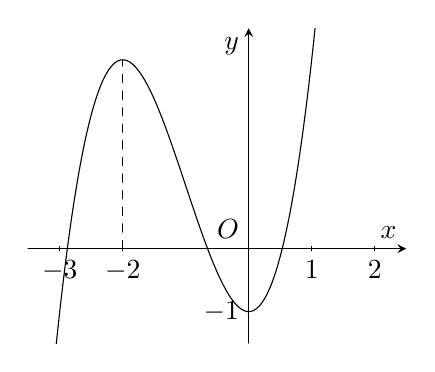
\begin{tikzpicture}[line cap=round,>=stealth,scale=0.8]
 %	\tikzset{every node/.style={scale=0.8}}
 \draw[->] (-3.5,0)--(2.5,0) node[above left] {$x$};
 \draw[->] (0,-1.5)--(0,3.5) node[below left] {$y$};
 \draw (0,0) node [above left] {$O$};
 \draw[dashed,thin](-2,0)--(-2,3) (0,-1) node[left] {$-1$};
 \foreach \x/\nx in {-3/-3, -2/ -2,1/1,2/2}
 \draw[thin] (\x,1pt)--(\x,-1pt) node [below] {$\nx$};
 \begin{scope}
 \clip (-3.5,-1.5) rectangle (2,3.5);
 \draw[samples=100,domain=-4.9:4.567,smooth,variable=\x] plot (\x,{1*((\x)^3)+3*((\x)^2)-1});
 \end{scope}
 \end{tikzpicture}
 }
 \loigiai{
 Nếu không quen nhìn đồ thị, ta có thể từ đồ thị thiết lập lại bảng biến thiên như sau:
 \begin{center}
 \begin{tikzpicture}
 \tkzTabInit[lgt=1,espcl=3]
 {$x$ /0.7, $y'$ /0.7, $y$ /2}
 {$-\infty$,$-2$,$0$,$+\infty$}
 \tkzTabLine{,+,$0$,-,$0$,+,}
 \tkzTabVar{-/$-\infty$,+/,-/$-1$,+/$+\infty$}
 \end{tikzpicture}
 \end{center}
 Suy ra
 \begin{itemchoice}
 \itemch Hàm số nghịch biến trên khoảng $(-2,0)$.
 \itemch Hàm số đồng biến trên khoảng $(0;+\infty)$ nên khẳng định đồng biến trên khoảng $(-1;+\infty)$ là sai.
 \itemch Hàm số đồng biến trên khoảng $(0;+\infty)$ nên nên hàm số đồng biến trên khoảng $(2;+\infty)$.
 \itemch Hàm số đạt cực tiểu tại $x=0$ (chú ý $y=-1$ gọi là giá trị cực tiểu).
 \end{itemchoice}
 }
\end{ex}
\begin{ex}
 Cho hàm số $y = f(x)$ xác định trên $\mathbb{R}$ và có đạo hàm $f'(x) = 3x^3 - 3x^2$, $\forall x\in \mathbb{R}$. Xét tính đúng sai của các khẳng định sau:
 \choiceTF
 {\True Hàm số đồng biến trên khoảng $(1;+\infty)$}
 {\True Hàm số nghịch biến trên khoảng $(-1;1)$}
 {Đồ thị hàm số có hai điểm cực trị}
 {\True Đồ thị hàm số có một điểm cực tiểu}
 \loigiai
 {
 Ta có: $y' = 0 \Leftrightarrow 3x^3 - 3x^2 = 0 \Leftrightarrow \hoac{& x = 0 \\& x = 1.}$\\
 Bảng biến thiên:
 \begin{center}
 \begin{tikzpicture}[>=stealth]
 \tkzTabInit[nocadre, lgt=1, espcl=2.5]
 {$x$ /0.7,$y'$ /0.7,$y$ /1.7}
 {$-\infty$,$0$,$1$,$+\infty$}
 \tkzTabLine{,-,$0$,-,$0$,+,}
 \tkzTabVar{+/ $+\infty$, R, -/{\text{CT}}, +/ $+\infty$}
 \end{tikzpicture}
 \end{center}
 Suy ra
 \begin{itemchoice}
 \itemch Hàm số đồng biến trên khoảng $(1;+\infty)$.
 \itemch Hàm số nghịch biến trên khoảng $(-\infty;1)$ nên nghịch biến trên $(-1;1)$.
 \itemch Hàm số có đúng một điểm cực trị.
 \itemch Hàm số có đúng một điểm cực tiểu $x = 1$.
 \end{itemchoice}
 }
\end{ex}
\begin{ex}%[Câu 15]%[2D1H2-1]
 Cho hàm số $y=f(x)=x^4-2x^2-3$. Xét tính đúng sai của các khẳng định sau:
 \choiceTF
 {\True Hàm số đã cho đạt cực đại tại $x=0$}
 {Hàm số đã cho đạt cực tiểu tại $x=-3$}
 {Hàm số đã cho có giá trị cực đại và cực tiểu lần lượt là $-4,-3$}
 {Đồ thị hàm số $g(x)=f(x)+3$ có điểm cực đại là $(0;0)$ }
 \loigiai{
 Ta có $y'=4x^3-4x$. Giải $y'=0$ ta được $x=-1$, $x=0$, $x=1$.\\
 Bảng biến thiên
 \begin{center}
 \begin{tikzpicture}
 \tkzTabInit[nocadre=false, lgt=1, espcl=2]
 {$x$ /0.7,$y'$ /0.7,$y$ /1.7}
 {$-\infty$,$-1$,$0$,$1$,$+\infty$}
 \tkzTabLine{,-,0,+,0,-,0,+,}
 \tkzTabVar{+/$-\infty$ ,-/ $-9$, +/ $-3$ /, -/$1$, +/$+\infty$}
 \end{tikzpicture}
 \end{center}
 \begin{itemchoice}
 \itemch Dựa vào bảng biến thiên ta thấy hàm số đạt cực đại tại $x=0$
 \itemch Dựa vào bảng biến thiên ta thấy hàm số đạt cực tiểu tại $x=-3$
 \itemch Dựa vào bảng biến thiên ta thấy hàm số giá trị cực đại và cực tiểu lần lượt là $-4,-3$
 \itemch Dựa vào bảng biến thiên ta thấy hàm số $g(x)=f(x)+3$ có được bằng cách tịnh tiến đồ thị $y=f(x)$ lên trên 3 đơn vị. Suy ra đồ thị hàm số $g(x)=f(x)+3$ có điểm cực đại là $(0;0)$.
 \end{itemchoice}
 }
\end{ex}
\BTTL
\begin{ex}
 Khoảng cách giữa hai điểm cực trị của đồ thị hàm số $y=-x^3+3x+2$ bằng bao nhiêu? (kết quả làm tròn đến hàng phần trăm)
 \shortans[3]{$4{,}47$}
 \loigiai{
 \begin{enumerate}[$ \star $]
 \item Tập xác định $\mathscr{D}=\mathbb{R}.$
 \item Đạo hàm $y'=-3x^2+3$.
 \item $y'=0\Leftrightarrow \hoac{&x=-1\Rightarrow y=0\\&x=1\Rightarrow y=4}$
 \item Bảng biến thiên
 \begin{center}
 \begin{tikzpicture}[>=stealth,line join=round, line cap=round, font=\footnotesize,scale=0.8]
 \tkzTabInit[nocadre=false,lgt=1.2,espcl=2.5,deltacl=0.6]
 {$x$/0.6,$y'$/0.6,$y$/2}
 {$-\infty$,$-1$,$1$,$+\infty$}
 \tkzTabLine{,-,0,+,0,-,}
 \tkzTabVar{+/$+\infty$,-/$0$,+/$4$,-/$-\infty$}
 \end{tikzpicture}
 \end{center}
 \item Hàm số đạt cực đại tại $x=1$, $y_{\textrm{CĐ}}=4$, suy ra $A(1;4)$.
 \item Hàm số đạt cực tiểu tại $x=-1$, $y_{\textrm{CT}}=0$, suy ra $B(-1;0)$.
 \item Khoảng cách giữa hai điểm cực trị của đồ thị hàm số là $AB=\sqrt{(1+1)^2+(4-0)^2}=2\sqrt{5} \approx 4{,}47$.
 \end{enumerate}
 }
\end{ex}
\begin{ex}
 Cho hàm số $ y=x^4-8x^2+10 $ có đồ thị $ (C) $. Gọi $ A,B,C $ là ba điểm cực trị của đồ thị $ (C) $. Tính diện tích $ S $ của tam giác $ ABC. $
 \shortans[3]{$32$}
 \loigiai{
 Ta có $ y'=4x^3-16x,y'=0\Leftrightarrow \hoac{&x=0\\&x=\pm 2} $.\\
 Tọa độ $ 3 $ điểm cực trị của đồ thị hàm số là $ A(0;10), B(-2;-6), C(2;-6)$.\\
 Gọi $ H $ là trung điểm $ BC \Rightarrow H(0;-6)$.\\
 Theo tính chất của hàm trùng phương nên tam giác $ ABC $ cân tại $ A .$\\
 Do đó $ S_{ABC}=\dfrac{1}{2}AH\cdot BC =\dfrac{1}{2}16\cdot 4=32. $
 }
\end{ex}
\begin{ex}%[Câu 20]%[2D1V1-3]
 Đồ thị hàm số $y=x^3-3x^2+2ax+b$ có điểm cực tiểu $A(2;-2)$. Khi đó $a+b$ bằng bao nhiêu?
 \shortans[3]{2}
 \loigiai{
 $y'=3x^2-6x+2a$.\\
 Ta có hệ phương trình
 $\heva{&4a+b=2 \\ &a=0} \Rightarrow \heva{&a=0 \\ &b=2.}$\\
 Vậy $a+b=2$.
 }
\end{ex}
\begin{ex}
 Có bao nhiêu giá trị nguyên của tham số $m$ để hàm số $y=-x^3-(m-1)x^2+3mx+1$ nghịch biến trên $\mathbb{R}$?
 \shortans[3]{6}
 \loigiai{
 Ta có $y'=-3x^2-2(m-1)x+3m$.\\
 Hàm số nghịch biến trên $\mathbb{R}$ khi $$y' \le 0 \, \forall x \in \mathbb{R} \Leftrightarrow \heva{& -3<0 \\ & \Delta' \le 0} \Leftrightarrow (m-1)^2-(-3)\cdot 3m \le 0 \Leftrightarrow \dfrac{-7-3\sqrt{5}}{2} \le m \le \dfrac{-7+3\sqrt{5}}{2}.$$
 Các giá trị nguyên của $m$ thỏa mãn là $-6$, $-5$, $-4$, $-3$, $-2$, $-1$.
 }
\end{ex}
\begin{ex}
 Có bao nhiêu giá trị nguyên của tham số $m$ để hàm số $y=\dfrac{-x+6}{x+m}$ đồng biến trên $(10;+\infty)$?
 \shortans[3]{4}
 \loigiai{
 Hàm số $y=\dfrac{-x+6}{x+m}$ có tập xác định: $\mathscr{D}=\mathbb{R}\setminus \{-m\}$ và đạo hàm $y'=\dfrac{-m-6}{(x+m)^2}$.\\
 Hàm số đồng biến trên khoảng $(10;+\infty)$ khi và chỉ khi $y'>0$, $\forall x\in (10;+\infty)$ \\
 \centerline{$\Leftrightarrow \left\{\begin{aligned}
 &-m-6>0\\
 &-m\leqslant 10\\
 \end{aligned}\right. \Leftrightarrow \left\{\begin{aligned}
 &m<-6\\
 &m\geqslant -10\\
 \end{aligned}\right. \Leftrightarrow -10\leqslant m<-6$.}
 Do $m\in\mathbb{Z}$ nên các giá trị của $m$ thoả mãn yêu cầu bài toán là $ m\in \{-10;-9;-8;-7\}$.}
\end{ex}
\begin{ex}
 Tìm giá trị thực của tham số $ m$ để đồ thị hàm số $ y=-x^3+3mx+1$ có hai điểm cực trị $A$, $B$ sao cho tam giác $OAB$ vuông tại $O$, với $O$ là gốc tọa độ.
 \shortans[3]{$0{,}5$}
 \loigiai{Đạo hàm $y'=-3x^2+3m=-3\left( x^2-m \right)$.\\
 Để hàm số có hai điểm cực trị $\Leftrightarrow x^2-m=0$ có hai nghiệm phân biệt $\Leftrightarrow m>0$.\\
 Tọa độ các điểm cực trị của đồ thị hàm số là $A\left( -\sqrt{m};1-2m\sqrt{m} \right)$ và $B\left( \sqrt{m};1+2m\sqrt{m} \right)$.\\
 Yêu cầu bài toán $\Leftrightarrow \overrightarrow{OA}.\overrightarrow{OB}=0\Leftrightarrow 4m^3+m-1=0\Leftrightarrow m=\dfrac{1}{2}$ (nhận).
 }
\end{ex}